\documentclass[11pt,a4paper]{article}
\usepackage[utf8]{inputenc}
\usepackage{amsmath,amssymb,amsthm}
\usepackage{booktabs}
\usepackage{hyperref}
\usepackage{geometry}
\usepackage{pgfplots}
\usepackage{orcidlink}
\pgfplotsset{compat=1.18}
\hypersetup{
  hidelinks,
  pdftitle={Independent Reproduction and Convergence Analysis of the Connes--Consani--Moscovici Zeta Spectral Triple},
  pdfauthor={Ronnie Andrews, Jr.},
  pdfsubject={Independent high-precision reproduction and convergence analysis of the CCM zeta spectral triple},
  pdfkeywords={Riemann zeta function, spectral triple, Weil quadratic form, high-precision computation, convergence}
}
\geometry{margin=1in}

\newtheorem{theorem}{Theorem}
\newtheorem{proposition}{Proposition}
\newtheorem{remark}{Remark}

\title{Independent Reproduction and Convergence Analysis\\
of the Connes--Consani--Moscovici Zeta Spectral Triple}

\author{Ronnie Andrews, Jr.\,\orcidlink{0009-0003-9724-3104}%
\thanks{Correspondence: \texttt{randrewsmath@gmail.com}}}

\date{June 2026\\[2pt]{\small Revised September 2026 (version 2.5)}}

\begin{document}
\maketitle

\begin{abstract}
We independently implement the Connes--Consani--Moscovici (CCM)
operator construction~\cite{CCM2025} in Rust at arbitrary precision
(MPFR/GMP) and extend the first-zero comparison from 55 to
\textbf{1495.14 measured matching decimal digits} at
$(\lambda^2{=}1200,N{=}970)$ with 6708 working bits.
At $(\lambda^2{=}1000,N{=}800)$, increasing requested precision from
HP-1000 to HP-2000 improves agreement from 1019.0 to 1260.36 digits,
separating arithmetic limitation from the resolved finite-configuration
error.
We characterize the construction's convergence empirically: accuracy
follows a smoothly saturating basis-size ramp that is approximately
linear over the observed early range, then approaches a first-zero
plateau that tracks the Weil eigenvalue depth
$-\log_{10}|\varepsilon_N|$ with a slowly varying conversion gap.
Along the sampled cutoff-and-basis paths, $|\varepsilon_N|$ decreases
by hundreds of decimal orders over the listed prime-count doublings,
although the finite data do not determine an asymptotic decay class.
Across the sampled fixed-$N$ cutoff sweep, first-zero accuracy grows
monotonically with~$\lambda$ and closely tracks the eigenvalue depth
$-\log_{10}|\varepsilon_N|$; no monotonicity claim is made outside
that range. The unrestricted lowest state is essentially even at every tested
above-floor configuration. At the five headline parity configurations,
positive even--odd and internal even-sector gaps additionally support
numerical simplicity. Analytic interval assembly and two independent
inertia calculations certify positive, simple, even ground states at
$\lambda^2=13$, $N=10$ and $N=120$. Propagating the analytic
eigenstate error also certifies the finite-source root comparisons at
these two configurations, including the 55-digit reproduction.
A residual-to-gap bound explains the observed
parity noise.
A $21\times21$ matrix from six primes already yields
$21.585$ matching digits; an exact reference-free census of its
serialized secular source verifies the root count and spectral indexing. All results are reproducible from the
accompanying source-available implementation. This work has been
shared with the CCM authors and reviewed by the lead author,
Professor Alain Connes.
\end{abstract}

\section{Introduction}

The Riemann Hypothesis (RH), asserting that all nontrivial zeros
of the Riemann zeta function $\zeta(s)$ satisfy $\Re(s) = 1/2$,
remains one of the central open problems in mathematics. Among
approaches toward its resolution, the Hilbert--P\'olya conjecture
--- positing the existence of a self-adjoint operator whose
spectrum encodes the imaginary parts of the nontrivial zeros ---
has motivated extensive work in spectral theory and noncommutative
geometry.

In November 2025, Connes, Consani, and Moscovici~\cite{CCM2025}
proposed the perturbed scaling-operator family
$D_{\log}^{(\lambda, N)}$, determined by a finite Weil-form restriction.
Its spectra exhibit striking
numerical agreement with the nontrivial zeros of $\zeta(1/2 + is)$ in the tested finite configurations.
Their construction uses the Weil quadratic
form built from the explicit formula, restricted to primes
$p \leq \lambda^2$, and produces a $(2N{+}1) \times (2N{+}1)$
self-adjoint matrix whose smallest eigenvalue $\varepsilon_N$
is observed to decrease over the tested families as $\lambda$ and $N$ increase. They reported
accuracy of $2.5 \times 10^{-55}$ on the first zero at
$(\lambda^2{=}13, N{=}120)$ with 200-digit working precision.
Subsequent independent work by Groskin reproduced the high-precision
zero approximation from the truncated Weil form across multiple
cutoffs~\cite{Groskin2026HighPrecision}.

Recent continuum results provide complementary context for the parity
observation below. Suzuki proves that, for sufficiently small compact-window
half-width $a>0$, the localized Weil operator has a positive, simple lowest
eigenvalue with an even eigenfunction~\cite{Suzuki2026WeilScrew}. Zhu reports
an unconditional certificate at $a=0.8$, equivalently
$\lambda^2=e^{2a}\approx4.95$, including a simple even continuum ground
state~\cite{Zhu2026CompactWeil}. The finite reduction, tail estimates,
and two-sector separation in that work provide a constructive route
from computed gaps to a continuum certificate. The numerical full-space
tests reported here begin at $\lambda^2=13$ and extend the tested
parameter range; quantitative tail and gap control is needed to connect
these finite tests to larger continuum windows. Zhu also
proposes a Landau--Widom-type decay law for the continuum compact-window
infimum, with a fitted leading constant. That proposal concerns a different
limit and is not used here as an asymptotic law for the finite Galerkin
quantity $\varepsilon_N(\lambda^2,N)$ or for secular-root error.

In this paper we:
\begin{enumerate}
\item Independently reproduce the CCM headline result on a
Rust + MPFR/GMP software stack;
\item Extend the first-zero comparison to
\textbf{1495.14 measured matching digits} at
$(C,N)=(1200,970)$, where $C=\lambda^2$. The paired-precision
experiment at $(C,N)=(1000,800)$ distinguishes arithmetic limitation
from finite-configuration error;
\item Systematically characterize the convergence behavior as a
function of both $N$ (basis size) and $\lambda$ (prime cutoff);
\item Test the simple-even ground-state condition using unrestricted
eigenvectors and the low spectra of both parity sectors. We give a
residual-to-gap estimate for parity error and an exact reference-free
root census for the small-matrix example.
\end{enumerate}

All computations are reproducible from the source-available
implementation at
\url{https://github.com/TeamXcelerator/ccm-reproduction-and-convergence}.

\section{Mathematical Setup}

We briefly recall the CCM construction, following the notation
of~\cite{CCM2025}.

\subsection{The Weil Quadratic Form}

Let $\lambda > 1$, $C=\lambda^2$, and $L = 2\ln\lambda=\ln C$. The Hilbert space is
$\mathcal{H}_\lambda = L^2([\lambda^{-1}, \lambda], du/u)$.
The finite Fourier subspace $E_N\subset\mathcal{H}_\lambda$ has
orthonormal basis
\[
V_n(u) = \frac{1}{\sqrt{L}}\,
e^{2\pi i n \ln(\lambda u)/L}, \quad
n \in \{-N, \ldots, N\}.
\]
The restriction of the Weil quadratic form $QW_\lambda$ to $E_N$
is represented by the real symmetric $(2N{+}1)\times(2N{+}1)$
matrix $\tau$ with entries
\[
\tau_{n,m} = W_{0,2}(V_n, V_m) - W_R(V_n, V_m)
- \sum_{\substack{k = p^j \\ k \leq \lambda^2}}
\frac{\log p}{\sqrt{k}}\, q(V_n, V_m)(\log k),
\]
where $W_{0,2}$ is a closed-form rank-two pole correction,
$W_R$ is the archimedean (gamma-factor) contribution computed
via Gauss--Legendre quadrature, and the prime-power sum encodes
the von Mangoldt function $\Lambda(k) = \log p$ for $k = p^j$.

\subsection{From Eigenvector to Spectral Ordinates}

Let $\varepsilon_N$ denote the smallest eigenvalue of $\tau$ and
$\xi=(\xi_{-N},\ldots,\xi_N)$ the corresponding eigenvector. In the
reproduction pipeline we analyze the even representative
($\xi_{-j}=\xi_j$) and normalize it so that
$\sum_j\xi_j=\sqrt{L}$. Define the secular rational function
\[
R(s)=\xi_0+2s\sum_{j=1}^{N}\frac{\xi_j}{s-j^2}.
\]
Let $s_1<\cdots<s_M$ denote its positive real roots, indexed in
increasing order. The corresponding positive spectral ordinates are
\[
\nu_r=\frac{2\pi}{L}\sqrt{s_r}.
\]
The root ordinal $r$ is not the pole-interval index $j$: many
intervals $(j^2,(j+1)^2)$ can be empty, and at small $N$ some roots
matching low zeta ordinates can lie above the largest pole $N^2$.
The full perturbed scaling operator agrees with the unperturbed
operator on $E_N^\perp$, retaining the lattice values
$2\pi j/L$ for $|j|>N$~\cite[Proposition~5.7]{CCM2025}.
We therefore distinguish the movable-root rank $r$, a reference-zero
label $k$, and the ordinal in the full positive spectrum. The tables
compare the selected roots with the ordered positive ordinates
$\gamma_k$ of $\zeta(1/2+i\gamma_k)=0$; identification by reference
matching is separate from counting the full spectrum. Section~4.4 gives
an exact count for the small example.

All tables reporting ``matching digits'' use the relative metric
\begin{equation}
D_r(\lambda^2,N,P)
:=-\log_{10}\!\left(\frac{|\nu_r-\gamma_r|}{|\gamma_r|}\right).
\label{eq:matching-digits}
\end{equation}
Section~\ref{sec:headline} also reports absolute error to compare
directly with the original CCM headline result.

\section{Implementation}

Our implementation uses the Xcelerator
Toolkit,\footnote{\url{https://github.com/TeamXcelerator/xcelerator-toolkit}}
a publicly available library of high-precision spectral methods for
analytic number theory, pinned to a tagged release for reproducibility.
The toolkit provides the core numerical primitives
(Gauss--Legendre quadrature with disk-cached HP nodes, LU-based
inverse iteration, Newton refinement) and the CCM-specific
construction (Weil-form matrix assembly, eigenvector extraction,
rational-function root-finding). The paper-specific repository contains
the CLI harness, reproduction scripts, and independent verification
supplements. The production numerical implementation is shared via
the toolkit.

The toolkit is built on:
\begin{itemize}
\item \textbf{Rust} (edition 2021) for the main codebase;
\item \textbf{rug} (v1.30, wrapping MPFR/GMP) for arbitrary-precision
floating-point arithmetic;
\item \textbf{nalgebra} (v0.33.3) for the f64 fast-path eigendecomposition
(used only by the optional \texttt{--f64-only} mode for smoke tests; the
HP publication path uses the toolkit's own HP symmetric eigendecomposition
in \texttt{xc-numerics::eigen}, verified at HP-1000 against a PARI/GP
2000-digit reference~\cite{PARI});
\item \textbf{rayon} (v1.12.0 in the locked dependency graph) for parallel
matrix assembly, Householder
reduction, LU factorization, and eigenvalue-per-seed refinement.
\end{itemize}

Key algorithmic choices:
\begin{enumerate}
\item \textbf{Parity-aware eigenstate solve:} Paper claims use the
direct reduced even-sector matrix. The default automatic solver first
reuses an exact compatible eigenstate when available; on a cache miss
it applies a retained-factor shift-invert Krylov/Rayleigh--Ritz method,
always initialized from its canonical state. Cache-derived or explicitly
supplied continuation states are not admitted to the persisted solve, so
the retained payload cannot depend on which compatible artifacts happened
to be present before the run. A
residual-verified LU inverse-iteration route remains the conservative
fallback when the targeted Ritz value is not isolated unambiguously.
The unrestricted natural and conditional-projection routes use the
full-space inverse-iteration implementation. Parity policy and solver
route are part of artifact identity, so numerically equivalent states
from different operation sequences cannot be confused in cache reuse.
\item \textbf{Halley's method for $R(s)$ zeros:} The rational
function $R(s)=\xi_0+2s\sum_{j=1}^{N}\xi_j/(s-j^2)$ has analytically
available first and second derivatives, enabling Halley's method
(cubic convergence) as the default root-finder. The paper-claim
scripts seed refinement from a toolkit-owned reference dataset whose
zeros were independently computed to 2,500 decimal digits using
rigorous Arb interval arithmetic~\cite{JohanssonArb}; their leading
1,000 digits were cross-validated against Odlyzko's
tabulation~\cite{Odlyzko}. The
reference ordinate selects which finite secular root is refined; it is
not substituted into the result. An accepted iterate must satisfy the
finite secular equation and the solver's convergence tests.
Independent finite-source discovery is also available for unseeded
research runs. The point solver distinguishes four outcomes:
\texttt{Converged} (the requested correction target was met),
\texttt{Stagnated} (a finite approximation stopped improving),
\texttt{Approximate} (the iteration limit was reached with a finite
value), and \texttt{Failed} (no usable finite value). Computed
workflows retain finite nonconverged values with diagnostics; they are
not mislabeled as converged or certified.
\item \textbf{Gauss--Legendre quadrature with disk cache:}
GL nodes and weights at a given quadrature order and bit precision
are computed once and cached for reuse across runs. This quadrature
evaluates the finite-$x$ representation of the full archimedean matrix
entries used by the CCM construction; it does not introduce the separate
finite-frequency cutoff $T$ used in Groskin's implementation and studied
there for truncation sensitivity~\cite{Groskin2026HighPrecision}.
\end{enumerate}

\paragraph{Independent matrix assembly.}
At $C=13$, $N=10$, a separate tanh--sinh integration of the defining
CCM components~\cite[Equations (3.14), (3.16), and (4.4)]{CCM2025}
checks all 441 entries, including the zero mode. The maximum absolute
differences from the analytic interval-assembly midpoints are
$4.05\times10^{-60}$ at 60 decimal digits and $2.95\times10^{-90}$
at 90 decimal digits. This independently checks the assembly formulas
numerically; the interval certificates below supply the rigorous
finite-matrix conclusions.

\subsection{Reproducibility Infrastructure}

The toolkit manages typed artifacts for quadrature rules, the
archimedean and prime components, $\tau$ matrices, parity reductions,
factorizations, Weil states, secular sources, root refinements, and
validation evidence. Each artifact has a content-bound manifest whose
semantic identity includes the numerical parameters, parity policy,
algorithm route, precision contract, and dependency identities that
can affect its value. Loads replay family-specific structural checks;
incompatible or obsolete artifacts are rejected rather than silently
reused.

Compatible artifacts are reused when available; otherwise, the
reproduction scripts compute them locally. Caching accelerates repeated
runs without changing the content-identified numerical route or the
validation checks. Reproducibility therefore does not depend on a
particular cached source being available.

The September 2026 v2.5 campaign assessed all 14 individual claim
scripts over 53 capture journals. Numerical and publication summaries
passed for every script, with the stated applicability policies.
Claim~1c retains five supported diagnostics and eight predeclared
exclusions. Claim~8 has a separate retrospective review of all four
journals and 46 applicable diagnostics; its original incomplete
natural-route receipts remain unchanged. The campaign summary
and supplemental numerical evidence are included in the repository's
\texttt{docs/RESEARCH\_EVIDENCE.md}.

\section{Results}

\subsection{Reproduction of the CCM Headline}
\label{sec:headline}

At $(\lambda^2{=}13,N{=}120,200\text{-digit precision})$, our first
computed spectral ordinate is
\[
\nu_1=14.134725141734693790457251983562470270784257\ldots
\]
(displayed truncated to $42$ digits; the full HP-1000 result has
$D_1=55.764$ under~\eqref{eq:matching-digits}, see
Section~\ref{sec:conv_N_label}) with absolute error
$2.4363\times10^{-55}$ against the independently computed 2,500-digit
reference. This matches the CCM paper's reported
$2.5\times10^{-55}$ to within rounding. The result is unchanged at an
HP-1000 requested-precision target, confirming that the observed
accuracy tracks $\varepsilon_N\approx3.48399\times10^{-59}$ rather
than being limited by arithmetic precision.

\subsection{Extension to 1019 Measured Digits}

\begin{table}[!htbp]
\centering
\caption{Measured matching digits across configurations, all at an
HP-1000 requested-precision target with a 64-bit internal guard reserve.
At $\lambda^2{=}1000$ the reported agreement saturates guarded working
precision; the construction's intrinsic ceiling is not resolved by this
run.}
\label{tab:headline}
\begin{tabular}{@{}lrrl@{}}
\toprule
Configuration & First-zero digits & 20th-zero digits & Requested precision \\
\midrule
$\lambda^2{=}13$,   $N{=}120$ & $55.764$  & $25.339$   & HP-1000 \\
$\lambda^2{=}100$,  $N{=}500$ & $460.09$ & $422.44$  & HP-1000 \\
$\lambda^2{=}1000$, $N{=}800$ & $\mathbf{1019.0}$ & $\mathbf{1020.3}$ & HP-1000 \\
\bottomrule
\end{tabular}
\end{table}

Here HP-1000 denotes the requested accuracy contract, not the raw MPFR
allocation. The implementation converts 1000 decimal digits to 3322
requested bits and appends 64 guard bits, giving 3386 working bits, or
approximately 1019.3 decimal digits. Root acceptance is tested against
the 3322-bit requested target; the guard reserve protects that target
from cancellation and accumulated rounding error. The matching-digits
diagnostic, however, compares the final values at the full guarded
precision, so a converged Halley iteration can expose agreement within
the reserve: 1019.0 digits for the first zero in the latest run. The
20th-zero relative metric reaches 1020.3. The bit-to-decimal conversion
describes significant arithmetic precision, not a strict upper bound on
pointwise agreement: a representable result can lie unusually close to
the comparison value. Division by $|\gamma_{20}|$ alone does not
explain this effect, since floating-point precision is already relative. These guard-space measurements do not
redefine HP-1000 as a 1019-digit requested calculation; they report the
additional agreement preserved by the internal working precision.

Increasing precision reveals additional digits while arithmetic
limits the root calculation. At the same
$(\lambda^2{=}1000,N{=}800)$, the HP-2000 run reaches 1260.36 matching
digits, rather than another full 1000 digits beyond the HP-1000 result.
The matrix scale, spectral gap, coefficient errors, and local secular
derivative determine how arithmetic error propagates to a root.
Cutoff, basis size, and working precision must therefore be budgeted
together for a desired root accuracy.

\subsection{\texorpdfstring{Convergence in $N$ (Basis Size)}
{Convergence in N (Basis Size)}}
\label{sec:conv_N_label}

\begin{table}[!htbp]
\centering
\caption{Matching digits on the first five zeros vs.\ $N$ at
$\lambda^2{=}13$. Values agree to the displayed precision at HP-200 and HP-1000 across
the entire sweep (see commentary below); the column shown is from
the HP-1000 run.}
\label{tab:conv_N}
\begin{tabular}{@{}rrrrrr@{}}
\toprule
$N$ & Zero 1 & Zero 2 & Zero 3 & Zero 4 & Zero 5 \\
\midrule
10  & $21.585$ & $16.335$ & $11.856$ & $5.1626$  & $3.4915$ \\
20  & $35.795$ & $32.261$ & $30.011$ & $26.504$ & $24.870$ \\
30  & $44.506$ & $41.267$ & $39.262$ & $36.208$ & $34.844$ \\
40  & $50.294$ & $47.152$ & $45.225$ & $42.304$ & $41.015$ \\
50  & $53.827$ & $50.721$ & $48.822$ & $45.948$ & $44.685$ \\
60  & $55.299$ & $52.203$ & $50.312$ & $47.451$ & $46.195$ \\
80  & $55.654$ & $52.560$ & $50.670$ & $47.811$ & $46.556$ \\
100 & $55.735$ & $52.641$ & $50.751$ & $47.892$ & $46.637$ \\
120 & $55.764$ & $52.670$ & $50.779$ & $47.921$ & $46.666$ \\
\bottomrule
\end{tabular}
\end{table}

The sweep shows a smoothly saturating ramp with two useful empirical
regimes:
\begin{enumerate}
\item \textbf{Rapid pre-saturation growth} ($N=10$ to
$N\approx60$): matching digits are approximately linear over the
early part of the sweep, while the local rate
$\Delta(\text{digits})/\Delta N$ decreases smoothly from
${\sim}1.4$ at $N{=}10{\to}20$ to ${\sim}0.15$ at
$N{=}50{\to}60$. The average ${\sim}0.96$ digits per unit $N$ over
$N\in[10,40]$ is a local summary, not a global rate law.
\item \textbf{Near-plateau behavior} ($N>60$): the first-zero
accuracy approaches $55.764$ digits by $N=120$. At this
configuration,
\[
D_{\varepsilon}:=-\log_{10}|\varepsilon_N|=58.458,
\]
so the first-zero plateau lies $2.694$ digits below the eigenvalue
depth. We therefore call it the root-accuracy plateau associated with
$\varepsilon_N$, not the eigenvalue depth itself.
\end{enumerate}

The precise local slope and plateau location are properties of the
sampled $(\lambda,N)$ regime. Here
$\lambda^2=13$ and $N\in\{10,20,30,40,50,60,80,100,120\}$; the paper does not
assert the same numerical break point at other cutoffs.

\begin{figure}[!htbp]
\centering
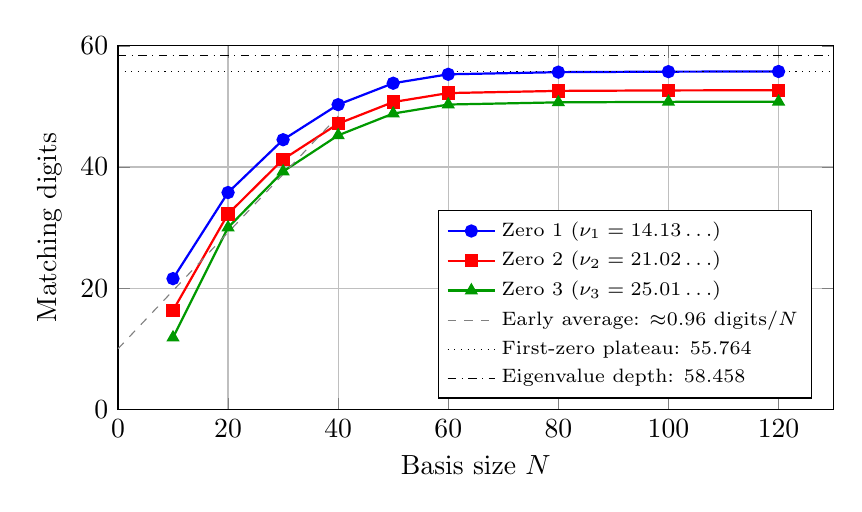
\begin{tikzpicture}
\begin{axis}[
    width=0.88\textwidth,
    height=6.2cm,
    xlabel={Basis size $N$},
    ylabel={Matching digits},
    legend pos=south east,
    legend style={font=\scriptsize},
    legend cell align={left},
    grid=major,
    xmin=0, xmax=130,
    ymin=0, ymax=60,
]
\addplot[blue, thick, mark=*] coordinates {
    (10, 21.585) (20, 35.795) (30, 44.506) (40, 50.294) (50, 53.827) (60, 55.299) (80, 55.654) (100, 55.735) (120, 55.764)
};
\addlegendentry{Zero 1 ($\nu_1=14.13\ldots$)}
\addplot[red, thick, mark=square*] coordinates {
    (10, 16.335) (20, 32.261) (30, 41.267) (40, 47.152) (50, 50.721) (60, 52.203) (80, 52.560) (100, 52.641) (120, 52.670)
};
\addlegendentry{Zero 2 ($\nu_2=21.02\ldots$)}
\addplot[green!60!black, thick, mark=triangle*] coordinates {
    (10, 11.856) (20, 30.011) (30, 39.262) (40, 45.225) (50, 48.822) (60, 50.312) (80, 50.670) (100, 50.751) (120, 50.779)
};
\addlegendentry{Zero 3 ($\nu_3=25.01\ldots$)}
\addplot[dashed, gray, domain=0:40] {0.96*x + 10};
\addlegendentry{Early average: ${\approx}0.96$ digits/$N$}
\addplot[dotted, black, domain=0:130] {55.764};
\addlegendentry{First-zero plateau: $55.764$}
\addplot[dashdotted, black, domain=0:130] {58.458};
\addlegendentry{Eigenvalue depth: $58.458$}
\end{axis}
\end{tikzpicture}
\caption{Convergence of matching digits vs.\ basis size $N$ at
$\lambda^2=13$, HP-1000. The two horizontal lines distinguish the
first-zero plateau from the deeper Weil-eigenvalue scale.}
\label{fig:conv_N}
\end{figure}

\paragraph{Precision comparison.}
At every $N$ in this sweep, HP-200 and HP-1000 produce matching digits that agree to the displayed precision. The observed plateau is therefore intrinsic to the
finite configuration rather than imposed by the arithmetic precision;
Sections~\ref{sec:lambda_convergence} and~\ref{sec:critical_N} describe
the corresponding floor mechanism in other regimes.

\subsection{\texorpdfstring{The 21-Digit Result from a $21\times 21$ Matrix}
{The 21-Digit Result from a 21 x 21 Matrix}}

At $N=10$ (matrix size $21\times21$), with only six primes
($\{2,3,5,7,11,13\}$, corresponding to nine prime powers entering
the Weil form), the first Riemann zero is matched to
\textbf{21.585 decimal digits}. This demonstrates notable numerical
compression: more than 21 matching digits from a $21\times21$ matrix.

This small configuration also illustrates that the lattice edge is not
a hard root cutoff. Here
\[
T_{\max}=\frac{2\pi N}{L}\approx24.50,
\]
yet the third through fifth zeta ordinates
$\gamma_3,\gamma_4,\gamma_5\approx25.01,30.42,32.94$ still have
accurate finite matches, and the corresponding secular roots lie above
the largest pole $N^2=100$. An exact reference-free census now makes this example more precise.
For the retained even state, interpret its serialized decimal
coefficients as exact rationals and clear the poles of $R(s)$.
The degree-ten numerator is squarefree, has no common factor with
$\prod_{j=1}^{10}(s-j^2)$, and has exactly ten positive real roots and
no negative roots. Exact Sturm isolation, independently replayed with
a second rational root counter, precedes the zeta comparisons.
Arb encloses the conversion to ordinates. The exact census first concerns the serialized finite source.
The error transfer in Proposition~\ref{prop:analytic_roots} additionally
certifies all ten root brackets for the analytic finite ground state.

\begin{table}[!htbp]
\centering
\caption{Reference-free census of the $C=13,N=10$ finite source.
The comparison labels coincide with the first five movable ranks.
Untouched scaling modes change the last two full-spectrum positions.}
\label{tab:small_census}
\begin{tabular}{@{}rrr@{}}
\toprule
Movable rank / reference label & Matching digits & Full positive ordinal \\
\midrule
1 & 21.585 & 1 \\
2 & 16.335 & 2 \\
3 & 11.856 & 3 \\
4 & 5.163 & 6 \\
5 & 3.491 & 8 \\
\bottomrule
\end{tabular}
\end{table}

For a nonlattice root, its full positive ordinal is
$r+\max\{0,\lfloor\sqrt{s_r}\rfloor-N\}$ in this counted source.
The third root lies above the retained Fourier edge but below the
first unchanged carrier. The fourth and fifth finite matches remain
valid and occupy positions six and eight. Thus the Fourier edge is
not an absolute boundary for a resolved finite-root match.

\subsection{\texorpdfstring{Rapid Empirical Change of $\varepsilon_N$}
{Rapid Empirical Change of epsilon-N}}
\label{sec:eps_n}

\begin{table}[!htbp]
\centering
\caption{Selected finite-configuration values of the smallest Weil
eigenvalue, with requested decimal precision and working bits.
All rows use the even-sector route. The explicit $N$ and precision
columns distinguish these values from floor-limited measurements.}
\label{tab:eps_N}
\begin{tabular}{@{}rrrrrr@{}}
\toprule
$\lambda^2$ & $N$ & Primes & HP / bits & $\varepsilon_N$ & Depth \\
\midrule
13   & 120 & 6   & 1000 / 3386 & $3.48399\times10^{-59}$   & $58.458$ \\
100  & 500 & 25  & 1000 / 3386 & $9.56481\times10^{-464}$  & $463.02$ \\
1000 & 800 & 168 & 2000 / 6708 & $3.92215\times10^{-1264}$ & $1263.41$ \\
\bottomrule
\end{tabular}
\end{table}

These values show a rapid increase in eigenvalue depth along the
listed finite-configuration path. They should not be read as a
prime-count-only law: the three rows use different basis sizes and sit
at different positions on the finite-$N$ ramp. The next table gives a
more systematic diagonal path with
$N/\sqrt{\lambda^2}\approx28$.

\begin{table}[!htbp]
\centering
\caption{Smallest Weil eigenvalue $\varepsilon_N$ above the
working-precision floor, with $N$ scaled at the fixed ratio
$N/\sqrt{\lambda^2}\approx28$. HP-1500 for $\lambda^2=500$--$800$
and HP-2000 for $\lambda^2=1000$--$1200$, with 5047 and 6708
working bits, respectively. The even-sector route is used throughout.
The $D_1$ column records the first-root matching digits retained by the
v2.5 campaign. The final column gives the
change in eigenvalue-depth digits, normalized per doubling of prime
count and computed between consecutive rows; it is illustrative rather
than a universal rate.}
\label{tab:eps_N_abovefloor}
\small
\begin{tabular}{@{}rrrrrrr@{}}
\toprule
$\lambda^2$ & $N$ & Primes & $\varepsilon_N$ & Depth & $D_1$ & Depth/doubling \\
\midrule
500  & 630 & 95  & $1.09117\times10^{-929}$  & $928.96$  & $925.938$ & --- \\
600  & 690 & 109 & $2.22999\times10^{-1029}$ & $1028.65$ & $1025.63$ & $502.6$ \\
700  & 740 & 125 & $9.45898\times10^{-1116}$ & $1115.02$ & $1112.00$ & $437.1$ \\
800  & 790 & 139 & $1.35946\times10^{-1199}$ & $1198.87$ & $1195.84$ & $547.4$ \\
1000 & 890 & 168 & $1.52095\times10^{-1362}$ & $1361.82$ & $1358.79$ & $596.1$ \\
1200 & 970 & 196 & $6.79867\times10^{-1499}$ & $1498.17$ & $1495.14$ & $613.1$ \\
\bottomrule
\end{tabular}
\end{table}

The depth grows rapidly throughout this sampled family. The per-doubling
numbers depend on the parameterization and, critically, on the chosen
basis path $N(\lambda)$. A different scaling of $N$ produces different
values. Six finite samples cannot establish whether the asymptotic
decay is polynomial, exponential, or super-exponential. A rigorous
two-parameter law for $\varepsilon_N(\lambda,N)$ remains open.

For the five retained even sources at $(C,N)=(13,120)$, $(100,500)$,
$(1000,800)$, $(1000,890)$, and $(1200,970)$, we additionally enclose
the first secular root using Arb and compare it with a freshly
computed rigorous zeta-zero enclosure. An independent replay verifies
opposite endpoint signs, pole exclusion, and a derivative that excludes
zero throughout each interval. The relative matching depths round to
$55.76$, $460.09$, $1260.36$, $1358.79$, and $1495.14$, respectively;
the final depth is enclosed by
$[1495.1385106984,1495.1385106986]$. These are certified local roots
of the exact serialized sources, including their finite decimal
coefficients. The analytic eigenstate error transfer is completed below for $C=13$.
The four larger-cutoff comparisons retain their serialized-source scope.

\subsection{\texorpdfstring{Observed Monotone Convergence in $\lambda$ at Fixed $N$}
{Observed Monotone Convergence in lambda at Fixed N}}
\label{sec:lambda_convergence}

At fixed $N=120$, first-zero accuracy grows monotonically across the
sampled cutoff range and closely tracks the eigenvalue depth
\[
D_{\varepsilon}(\lambda):=-\log_{10}|\varepsilon_N(\lambda)|.
\]
The two quantities are not identical: their difference is the
finite eigenvalue-to-root conversion gap.

\begin{table}[!htbp]
\centering
\small
\caption{First-zero accuracy vs.\ $\lambda^2$ at $N=120$, comparing
HP-200 and HP-1000 requested precision. The final column shows the
slowly varying conversion gap
$C_{\mathrm{conv}}=D_{\varepsilon}-D_1$.}
\label{tab:lambda_sweep}
\begin{tabular}{@{}rrlrrr@{}}
\toprule
$\lambda^2$ & Primes & $\varepsilon_N$ at HP-1000 & HP-200 & HP-1000 & $C_{\mathrm{conv}}$ \\
\midrule
13  & 6  & $3.48399\times10^{-59}$  & $55.764$ & $55.764$ & $2.694$ \\
20  & 8  & $2.50471\times10^{-96}$  & $92.817$ & $92.817$ & $2.784$ \\
30  & 10 & $2.19404\times10^{-135}$ & $131.80$ & $131.80$ & $2.859$ \\
50  & 15 & $6.89051\times10^{-174}$ & $170.19$ & $170.19$ & $2.972$ \\
100 & 25 & $3.48656\times10^{-215}$ & $211.29$ & $211.29$ & $3.168$ \\
\bottomrule
\end{tabular}
\normalsize
\end{table}

For HP-200, the implementation converts the 200-decimal-digit request
to 665 bits and adds 64 guard bits, yielding 729 working bits, or
approximately 219.5 decimal digits. Root acceptance is still measured
against the 665-bit requested target. The 211.29-digit result at
$\lambda^2=100$ therefore uses part of the guard reserve without
changing the nominal HP-200 accuracy contract. Diagnostics closer to
the floor remain precision-sensitive: HP-200 gives
$\varepsilon_N=3.48676\times10^{-215}$, compared with
$3.48656\times10^{-215}$ at HP-1000. For the retained complete-QR sector comparison, define
$\mathrm{GapLog}=\log_{10}(|o_0|/|e_0|)$, where $e_0,o_0$ are the
lowest even and odd values. Its values are $4.246343$ and $4.246284$
at 729 and 3386 bits, respectively. The full retained inputs reproduce
these diagnostics; operation-route identities distinguish their
low-precision variants.

Two empirical regularities emerge:
\begin{enumerate}
\item \textbf{Observed monotone growth over the sampled range.}
First-zero accuracy increases at every listed cutoff. No fixed-$N$
monotonicity claim is made outside this finite sweep.
\item \textbf{$\varepsilon_N$-tracked root accuracy.}
The first-zero digits follow $D_{\varepsilon}$ with a conversion gap
that grows slowly from about $2.7$ to $3.2$ digits across the table.
\end{enumerate}

The cutoff dependence is not featureless. Each prime-power threshold
changes the finite matrix path and produces a localized slope kink,
precisely the event structure isolated by
Groskin~\cite{Groskin2026MatrixVonMangoldt}. In sampled accuracy and
eigenvalue curves these events appear as fine-scale perturbations on
an otherwise smooth envelope, rather than as a separate staircase law.

For practitioners, increasing the cutoff is useful only when basis
size and working precision are scaled with the desired target. The
present sweep establishes monotone growth only for
$13\leq\lambda^2\leq100$ at $N=120$; it does not assert that increasing
$\lambda$ alone is sufficient outside that range.

\subsection{\texorpdfstring{Critical $N$ at Fixed Working Precision}
{Critical N at Fixed Working Precision}}
\label{sec:critical_N}

Critical $N$ must specify the criterion being met. Resolving a requested
root, reaching a specified accuracy, and entering a regime where cutoff
or numerical precision limits further improvement are distinct events.
Their basis requirements depend on the cutoff, the selected root, and
the working precision; an accuracy threshold also depends on the
requested matching depth.

Here we report a target-accuracy threshold on a tested ladder
$\mathcal N$, holding cutoff and precision fixed. For root index $r$
and requested depth $D_*$, define
\[
N_{\mathrm{crit,tested}}(D_*;r)
 =\min\{N\in\mathcal N:D_r(N)\ge D_*\},
\]
with $D_r$ assessed only where the requested root match is resolved.
If no tested configuration qualifies, the target is not reached on
that ladder. This is the first successful sampled value, not a
certified minimum over every integer $N$ or a guarantee for all larger
bases. A persistent threshold requires additional monotonicity or
uniform error bounds.

\begin{table}[!htbp]
\centering
\caption{Large-basis configurations at HP-1000, reporting the smallest
Weil eigenvalue and first- and fifth-zero matching digits. These paired
measurements show gains with increasing $N$; they do not locate exact
critical basis sizes.}
\label{tab:critical_N}
\begin{tabular}{@{}lrrr@{}}
\toprule
Configuration & $\varepsilon_N$ at HP-1000 & First-zero digits & 5th-zero digits \\
\midrule
$\lambda^2{=}50$, $N{=}200$  & $5.69795\times 10^{-221}$ & $217.34$ & $207.24$ \\
$\lambda^2{=}50$, $N{=}250$  & $4.51247\times 10^{-239}$ & $235.45$ & $225.42$ \\
$\lambda^2{=}100$, $N{=}300$ & $4.68074\times 10^{-368}$ & $364.37$ & $354.03$ \\
$\lambda^2{=}100$, $N{=}400$ & $6.12702\times 10^{-423}$ & $419.28$ & $409.04$ \\
\bottomrule
\end{tabular}
\end{table}

Table~\ref{tab:conv_N} supplies concrete sampled thresholds at
$\lambda^2=13$. The coarse ladder first reaches 50 matching digits at
$N=40$ and 55 digits at $N=60$. To resolve these crossings, we tested
every integer in $31\leq N\leq40$ and $51\leq N\leq60$ at both
HP-200 and HP-1000 (40 additional computations). The denser ladder
retains the 50-digit threshold at $N=40$ and refines the 55-digit
threshold to $N=56$; Table~\ref{tab:critical_brackets} gives the
adjacent pairs. Every tested value before each crossing falls below
its target, and every tested value from the crossing to that bracket's
upper endpoint meets it. The maximum difference in matching depth
between the two precisions is less than $3.18\times10^{-160}$ digits.

\begin{table}[!htbp]
\centering
\caption{Adjacent-integer Critical-$N$ crossings at $C=13$ for the
first zero. HP-200 and HP-1000 agree at all digits shown. The tested
integer brackets are $31$--$40$ and $51$--$60$, respectively.}
\label{tab:critical_brackets}
\begin{tabular}{@{}rrrrr@{}}
\toprule
Target & Preceding $N$ & $D_1$ & First passing $N$ & $D_1$ \\
\midrule
50 digits & 39 & 49.745584 & 40 & 50.293684 \\
55 digits & 55 & 54.708183 & 56 & 55.011854 \\
\bottomrule
\end{tabular}
\end{table}

By contrast, the
early average of approximately $0.96$ digits per added mode does not
justify extrapolating to 200 matching digits at $N\approx210$: the
slope decreases substantially, and the observed first-zero agreement
is only $55.764$ digits at $N=120$. This finite sweep also does not
establish an infinite-$N$ accuracy ceiling.

Table~\ref{tab:critical_N} shows that other cutoffs and larger bases
reach substantially greater depths at HP-1000. To distinguish an
accuracy threshold from the onset of saturation, one must compare
basis-size sweeps at sufficient precision and check precision
sensitivity at fixed configurations. Extra modes alone need not meet
a target when cutoff or numerical error remains limiting.

The companion convergence study~\cite{Andrews2026ConvergenceLaw} develops
the joint basis, cutoff, and precision budget.

\subsection{Even-Symmetry of the Smallest Eigenvector}
\label{sec:evenness}

The simple-even ground-state condition in the CCM program motivates
two finite tests: the parity of the unrestricted lowest state and its
separation from the lowest odd and next even states. Let $J$ denote
the corresponding coefficient reversal, $(J\xi)_j=\xi_{-j}$. We
measure the natural evenness $\|\xi-J\xi\|/\|\xi\|$ of the
unforced smallest eigenvector at working precisions sufficient to
resolve $\varepsilon_N$ above the floor:

\begin{table}[!htbp]
\centering
\caption{Symmetry properties of the natural (unforced) smallest
eigenvector, each measured at working precision sufficient to
resolve $\varepsilon_N$ above the floor. At every configuration
tested, the natural eigenvector is essentially even and the
natural and even-sector eigenvalues agree to hundreds of decimal
digits.}
\label{tab:evenness}
\begin{tabular}{@{}rrrlll@{}}
\toprule
$\lambda^2$ & $N$ & Precision & Evenness deviation & Eigenvalue rel.\ diff. & Verdict \\
\midrule
13    & 120  & HP-1000  & $2.126 \times 10^{-966}$  & $1.107 \times 10^{-962}$ & essentially even \\
100   & 500  & HP-1000  & $6.665 \times 10^{-563}$  & $2.444 \times 10^{-559}$ & essentially even \\
1000  & 800  & HP-2000  & $7.634 \times 10^{-763}$  & $1.559 \times 10^{-758}$ & essentially even \\
1000  & 890  & HP-2000  & $1.563 \times 10^{-664}$  & $1.807 \times 10^{-660}$ & essentially even \\
1200  & 970  & HP-2000  & $2.948 \times 10^{-528}$  & $7.927 \times 10^{-526}$ & essentially even \\
\bottomrule
\end{tabular}
\end{table}

The retained sector spectra supply the simplicity test. Let $e_0,e_1$
be the first two even-sector eigenvalues and $o_0$ the lowest odd one.
All five configurations have $e_0>0$, $o_0-e_0>0$, and $e_1-e_0>0$.
The odd-to-even ground-value ratio ranges from $8.77\times10^3$ to
$4.21\times10^5$. Independently retained HP Sturm brackets separate
the first two even indices, and the even-state residual divided by
that separation is below $2.01\times10^{-533}$ in every row.
The two sector spectra and the response record are bound to a common
Tau source. Together with the unrestricted states, these measurements
support both simplicity and evenness of the finite ground state.

\begin{table}[!htbp]
\centering
\small
\caption{Computed ground-state separations at the precisions of
Table~\ref{tab:evenness}. The last column is the even-state absolute
residual divided by the computed same-sector separation. These HP
values are numerical evidence, not analytic-matrix interval certificates.}
\label{tab:sector_separations}
\begin{tabular}{@{}rrrrr@{}}
\toprule
$\lambda^2$ & $N$ & $o_0-e_0$ & $e_1-e_0$ & Residual / gap \\
\midrule
13 & 120 & $3.05556\times10^{-55}$ & $1.31185\times10^{-51}$ & $1.13209\times10^{-968}$ \\
100 & 500 & $1.79801\times10^{-458}$ & $1.78543\times10^{-453}$ & $2.70026\times10^{-567}$ \\
1000 & 800 & $1.24493\times10^{-1258}$ & $2.05363\times10^{-1253}$ & $6.60626\times10^{-768}$ \\
1000 & 890 & $5.42414\times10^{-1357}$ & $1.04167\times10^{-1351}$ & $1.55669\times10^{-669}$ \\
1200 & 970 & $2.86128\times10^{-1493}$ & $6.55282\times10^{-1488}$ & $2.00727\times10^{-533}$ \\
\bottomrule
\end{tabular}
\end{table}

\paragraph{Certified finite ground states.}
At $C=13$, $N=10$ and $N=120$, we additionally assembled the analytic
cutoff-free matrix in interval arithmetic, using 512 and 1024 bits,
respectively. Arb interval $LDL^T$ proves positive definiteness of
the full matrix and encloses $e_0,e_1,o_0$ by shifted inertia.
The parity restrictions use the exact reflection symmetry and integer
bases, with diagonal mass matrices, avoiding rounded normalization
factors. Each bracket isolates exactly one sector eigenvalue, and
$\sup I_{e_0}<\min\{\inf I_{e_1},\inf I_{o_0}\}$ proves that the
full ground state is simple and even. Table~\ref{tab:finite_certificates}
reports the certified controls. A second implementation, using
Schur updates, wider entry enclosures, and direct basis contractions,
independently reproduces every inertia count at 500 decimal digits.
These certificates concern the analytic finite matrices; a continuum
extension also requires bounds on the omitted tail and coupling.
They are separate verification supplements, not certificates inferred
from Ultra capture receipts.

\begin{table}[!htbp]
\centering
\caption{Certified finite controls at $C=13$. Displayed centers locate
the exact rational brackets supplied with the verification supplement;
each bracket has relative half-width $10^{-6}$. Both full matrices
are positive definite, with a simple even ground state.}
\label{tab:finite_certificates}
\begin{tabular}{@{}rrrr@{}}
\toprule
$N$ & $e_0$ & $o_0$ & $e_1$ \\
\midrule
10 & $2.83124\times10^{-26}$ & $1.64492\times10^{-23}$ & $5.49026\times10^{-21}$ \\
120 & $3.48399\times10^{-59}$ & $3.05591\times10^{-55}$ & $1.31185\times10^{-51}$ \\
\bottomrule
\end{tabular}
\end{table}

The $\lambda^2{=}100$, $N{=}500$ row was remeasured with the current
64-bit guard reserve; the earlier 16-guard-bit calculation gave
$5.102\times10^{-548}$. The additional 48 working bits supply
approximately $48\log_{10}2=14.45$ decimal digits of arithmetic
headroom, consistent with the roughly 15-order reduction to
$6.665\times10^{-563}$. This change lowers the residual symmetry noise
without changing the smallest eigenvalue, its sign, or the
``essentially even'' conclusion; the natural and even-sector
eigenvalues differ by only $2.444\times10^{-559}$ in relative terms.

The $\lambda^2{=}1000$ rows show the same guard-reserve effect. At
$N{=}800$ the deviation falls from the earlier
$2.941\times10^{-748}$ to $7.634\times10^{-763}$, and at $N{=}890$
from $6.279\times10^{-650}$ to $1.563\times10^{-664}$. Both
improvements are approximately $14.6$ decimal orders, consistent
with the added 48 guard bits. The relative natural-versus-even
eigenvalue differences are $1.559\times10^{-758}$ and
$1.807\times10^{-660}$, respectively, so the two routes remain
numerically equivalent to hundreds of decimal digits.

The $\lambda^2{=}1200$, $N{=}970$ row was likewise remeasured with
the 64-bit guard reserve. Its evenness deviation falls from
$2.927\times10^{-514}$ to $2.948\times10^{-528}$, an improvement of
approximately $14.0$ decimal orders. The natural and even-sector
eigenvalues are numerically equivalent at the attainable relative
precision, agreeing to approximately 525 decimal digits with relative
difference $7.927\times10^{-526}$. Their full 6708-bit
representations need not be bit-identical: the natural full-space
solve and the reduced even-sector solve follow different high-precision
operation sequences, so roundoff at the working-precision floor need
not produce identical terminal bit patterns.
Moreover, 6708 bits provide approximately 2019 decimal digits, while
$|\varepsilon_N|\approx 6.799\times10^{-1499}$ consumes roughly 1499
orders of magnitude; the resulting ${\sim}520$ relative-digit
headroom is consistent with the observed 525-digit agreement. Thus
the nonzero difference reflects the arithmetic floor rather than a
mathematical discrepancy between the two eigenvalues.

At every configuration tested above the precision floor --- including
$\lambda^2 = 1200$, far beyond the range previously reported --- the
natural smallest eigenvector is even to hundreds of digits of precision,
and the natural and even-sector solves converge to numerically
indistinguishable eigenvalues at the reported accuracy. In the current
$\lambda^2{=}13$, $N{=}120$, HP-1000 reproduction, performed at 3386-bit
working precision, their relative difference is
$1.107 \times 10^{-962}$. The unrestricted states and the two positive gaps provide empirical
support for the finite simple-even hypothesis at these five
configurations. We conjecture the same structure throughout the finite
family: for every $\lambda>1$ and $N\geq1$, the lowest eigenspace of
$QW_\lambda|_{E_N}$ is one-dimensional and even.

\begin{proposition}[Residual control of parity]
\label{prop:parity_residual}
Let $A=A^*$ commute with an orthogonal involution $J$, let
$\|v\|_2=1$, let $\rho\in\mathbb{R}$, and set $r=Av-\rho v$.
If $\rho$ lies below the odd-sector spectrum by a distance at least
$g_o>0$, then
\[
\|v-Jv\|_2\leq \frac{2\|r\|_2}{g_o}.
\]
\end{proposition}
\begin{proof}
With $v_-=(I-J)v/2$, the odd projection gives
$(A_--\rho I)v_-=r_-$, where $A_-$ is the odd restriction.
Its inverse has norm at most $g_o^{-1}$, so
$\|v-Jv\|_2=2\|v_-\|_2\leq2\|r\|_2/g_o$.
\end{proof}

For the natural solver's stored infinity-relative residual
$r_\infty=\|Av-\rho v\|_\infty/\|v\|_\infty$, a two-norm estimate is
$\sqrt{2N+1}\,r_\infty\|v\|_\infty/\|v\|_2$.
Together with the measured odd gaps, this gives parity upper estimates
of $4.61\times10^{-964}$, $1.84\times10^{-560}$,
$3.20\times10^{-760}$, $1.23\times10^{-661}$, and
$8.14\times10^{-526}$ in table order. Every measured parity defect
lies below its corresponding estimate. This is a computed consistency
check; certified residuals and gaps would turn the same calculation
into a verified bound for the analytic matrix.
If stored entries only approximately commute with reflection, the
matrix-symmetry error must also enter the residual budget.

The proposition identifies the absolute gap, rather than the
odd-to-even eigenvalue ratio alone, as the conditioning scale for
parity. If $\|r\|_2\leq K(\lambda,N)2^{-P_{\rm bits}}$, then parity
tolerance $\eta$ follows from
$P_{\rm bits}\geq\log_2(2K/(\eta g_o))$.
This is a conditional precision budget once $K$ and $g_o$ are bounded,
and does not by itself give a root-accuracy budget.

\begin{proposition}[Transfer to analytic finite roots]
\label{prop:analytic_roots}
Let $q$ be an exact real unit approximate state and let the real
symmetric matrix $A$ have a simple ground state $u$. Suppose a real shift $\rho$ lies
below the remaining spectrum by at least $g>0$. Put
$R=\|Aq-\rho q\|_2$ and assume $R/g<1$. After aligning the sign of
$u$ with $q$, one has
\[
\|u-q\|_2\leq\eta:=\sqrt{2}\,R/g.
\]
For $H_q(t)=\sum_jq_j/(t-h_j)$, away from the poles,
\[
|H_u(t)-H_q(t)|\leq\eta\Bigl(\sum_j|t-h_j|^{-2}\Bigr)^{1/2},
\qquad
|H'_u(t)-H'_q(t)|\leq\eta\Bigl(\sum_j|t-h_j|^{-4}\Bigr)^{1/2}.
\]
Opposite endpoint signs and a derivative separated from zero after
these error budgets are included certify a unique root of $H_u$.
\end{proposition}
\begin{proof}
Spectral decomposition bounds the component of $q$ orthogonal to
$u$ by $R/g$. If its norm is $\sin\theta$, then the aligned unit
vectors satisfy $\|u-q\|_2\leq\sqrt{2}\sin\theta$.
The two function bounds follow from Cauchy--Schwarz. Continuity
and the derivative bound give existence and uniqueness of the root.
For an exactly even $q$, the same argument can use the remaining
even-sector spectrum.
\end{proof}

At $C=13$, the analytic interval matrices give
$\eta<3.83\times10^{-130}$ for $N=10$ and
$\eta<2.23\times10^{-242}$ for $N=120$. With these errors included,
all ten $N=10$ brackets and the $N=120$ bracket near $\gamma_1$
pass the endpoint and derivative tests. The first five $N=10$
comparisons retain the matching depths in Table~\ref{tab:small_census};
the $N=120$ comparison has
$D_1\in[55.7635578784,55.7635578796]$.
For $N=10$, ten distinct positive roots exhaust a numerator of
degree at most ten, so the complete count and the stated full-spectrum
ordinals transfer to the analytic finite source. An independent
calculation using wider matrix enclosures, an infinity-norm residual
bound, and the smaller full-space spectral gap verifies all eleven
brackets. These are finite CCM results, without taking a continuum
or increasing-cutoff limit.

\paragraph{Fixed-matrix precision control.}
We round one fixed $C=13$, $N=10$ matrix to 24, 53, 64, 80, 96,
128, 192, 256, and 384 bits, then solve each rounded problem at
220 decimal digits. This separates matrix-entry rounding from
assembly and solver precision. At 24 bits the lowest state is odd,
so the even-source root comparison is inapplicable. At 53 and 64
bits the lowest eigenvalue is negative, with first-zero matching
depths of 16.971 and 17.759 digits. At 192 bits and above the
positive ground value and 21.585231815758-digit match are recovered.
Thus entry rounding alone can produce the apparent failure and its
recovery; the threshold is specific to the configuration.

\paragraph{The precision-floor artifact.}
When $|\log_{10}\varepsilon_N|$ approaches or exceeds the working
precision in digits, the eigenvalue sinks below the arithmetic's
resolving power. In this regime the computed eigenvector is
under-resolved and becomes sensitive to rounding within numerically
indistinguishable directions. The result can \emph{appear} non-even
(deviation $\sim O(1)$), while the eigenvalues can \emph{appear} to
split between the natural and even-sector paths. Under the earlier
guard policy, the HP-1000 $\lambda^2 = 1000$ configuration
($|\log_{10}\varepsilon_N| \approx 1264$, well past the available
arithmetic floor) exhibits this artifact: deviation $1.87$, eigenvalue
split $24\%$. Increasing the requested precision to HP-2000 under the
same policy at the \emph{identical} $(\lambda^2{=}1000, N{=}800)$
configuration collapses the apparent breakdown entirely: deviation
$2.94 \times 10^{-748}$, with eigenvalues numerically equivalent at the
reported precision. Thus the only
variable in that controlled comparison is requested precision. The
latest 64-guard-bit HP-2000 run uses 6708 working bits (approximately
2019.3 decimal digits, a floor ratio of approximately $1.60$) and
reduces the residual symmetry noise further to
$7.634 \times 10^{-763}$, again with numerically equivalent natural and
even-sector eigenvalues at the reported precision.

\paragraph{The even-sector restriction is empirically unnecessary.}
To further test whether the eigenvector is naturally even, we ran
the full CCM pipeline (eigenstate solve $\to$ eigenvector $\to$
$R(s)$ zero-finding $\to$ Riemann-zero matching digits) with the
unrestricted natural full-space policy at configurations spanning
$\lambda^2 = 13$--$1000$, $N = 10$--$800$, and HP-200 through
HP-2000. At every tested above-floor point, the natural path produces
eigenvalues and Riemann-zero approximations numerically
indistinguishable from the reduced even-sector path at the reported
accuracy. The direct restriction is therefore not needed to obtain
the reported values at these points, although it remains the faster
paper-reproduction default.

\section{Discussion}

\subsection{Where the Construction's Power Lies}

The CCM construction's measured accuracy is controlled jointly by
three caller-selected parameters:
\begin{itemize}
\item $\lambda$ sets the arithmetic cutoff and changes the intrinsic
finite-configuration depth;
\item $N$ controls progress along the finite-basis ramp toward that
depth;
\item working precision determines how much of the finite result can be
resolved without floor artifacts.
\end{itemize}

Along the sampled path $N/\sqrt{\lambda^2}\approx25$--$30$, the
HP-2000 runs at $(\lambda^2,N)=(1000,890)$ and $(1200,970)$ achieve
1358.79 and 1495.14 first-root matching digits, respectively. These
are achieved finite accuracies, distinct from the requested precision.
The ratio is not a universal budget for reaching the finite-cutoff plateau: Tables~\ref{tab:eps_N_abovefloor} and
\ref{tab:critical_N} still show substantial gains from additional
modes beyond that ratio. A companion convergence-law study
\cite{Andrews2026ConvergenceLaw} examines the broader coordinate
$N/(\lambda^2\ln\lambda^2)$; the present reproduction paper does not
assume that model. In practice, $\lambda$, $N$, and precision should be
chosen together for the desired accuracy target.

\subsection{The Prime-Weight Profile}

Each prime power $k = p^j$ contributes weight
$\Lambda(k)/\sqrt{k} = \log(p)/\sqrt{k}$ to the Weil form. For
primes ($j=1$), this is $\log(p)/\sqrt{p}$, whose derivative
vanishes at $p = e^2 \approx 7.3891$ with maximum value
$2/e \approx 0.73576$.

\begin{table}[!htbp]
\centering
\caption{Individual prime contributions $\log(p)/\sqrt{p}$ for the
primes captured by $\lambda^2 = 13$. The maximum value $2/e$ is
attained at the (non-prime) point $p = e^2 \approx 7.3891$;
the integer prime $7$ achieves $99.96\%$ of this maximum.}
\label{tab:prime_contributions}
\begin{tabular}{@{}rrr@{}}
\toprule
$p$ & $\log(p)/\sqrt{p}$ & \% of $2/e$ \\
\midrule
2  & $0.49013$ & $66.62\%$ \\
3  & $0.63428$ & $86.21\%$ \\
5  & $0.71976$ & $97.83\%$ \\
\textbf{7}  & $\mathbf{0.73548}$ & $\mathbf{99.96\%}$ \\
11 & $0.72299$ & $98.26\%$ \\
13 & $0.71139$ & $96.69\%$ \\
\midrule
\multicolumn{2}{r}{$\max = 2/e$ at $p = e^2$} & $100\%$ \\
\bottomrule
\end{tabular}
\end{table}

The following observation describes a property of the resulting finite prime set; it does not imply that the original cutoff was selected for this reason.

The CCM paper's choice of $\lambda^2 = 13$ has the useful consequence
that it captures the peak prime $p = 7$ to within $0.04\%$ of the
maximum value and includes
both adjacent primes ($p = 5$ at $97.8\%$ of the maximum and
$p = 11$ at $98.3\%$) that lie within $\sim 2\%$ of the peak. The
choice covers the entire near-peak cluster of primes.

Past the peak, $\log(p)/\sqrt{p}$ decays as a power law with a
logarithmic factor ($0.46052$ at $p = 100$, $0.21844$ at $p = 1000$,
$0.092103$ at $p = 10000$). Thus later primes still have visible
individual weights at the finite cutoffs studied here. Their
cumulative effect is consistent with the measured reduction in
$|\varepsilon_N|$, but the scalar weight profile alone does not derive
the eigenvalue-decay law; matrix interactions and the simultaneous
scaling of $N$ remain essential.

\paragraph{Measured prime-power responses.}
At $C=13$, $N=120$, we independently test each retained prime-power
matrix direction $D_q$ by solving the perturbed family $A+tD_q$ with
fixed observation poles. All nine directions pass at
$t=10^{-90},10^{-100},10^{-110}$. Centered-difference errors decrease
quadratically; the final relative discrepancies in first-root velocity
are below $1.1\times10^{-117}$. Powers 2, 3, 5, and 7 contribute
approximately $-226.280$, $-16.1755$, $-3.15035\times10^{-4}$, and
$-1.71768\times10^{-10}$, respectively. The scalar weight maximum
at 7 therefore does not identify the largest local root response.

The source-matched retained decomposition contains approximately
$+274.545$ from the pole-correction matrix, $-26.5174$ from the
archimedean matrix, $-242.517$ from the aggregate prime matrix,
and $-5.51072$ from moving secular poles. Their full-precision sum is
$-4.61362\times10^{-53}$; the rounded displayed components cannot
reproduce that cancellation. The aggregate is reconciled from
retained measurements, rather than an independent validation of
every nonprime derivative. A separate one-sided matrix check also
verifies the prime-13 activation derivative. These results identify
local response and cancellation, not finite prime-removal effects
or an asymptotic convergence law.

\subsection{Implications for the Proof Strategy}

Our findings have implications for the CCM proof strategy:
\begin{enumerate}
\item The unrestricted evenness measurements and both spectral gaps
(Tables~\ref{tab:evenness} and~\ref{tab:sector_separations}) support a
simple even finite ground state through $\lambda^2=1200$ at HP-2000.
The corresponding conjecture has a concrete certification target:
strict separation of the first even value from the next even and
lowest odd values. The two finite instances in
Table~\ref{tab:finite_certificates} now meet that target rigorously.
Proposition~\ref{prop:parity_residual} connects
observed parity noise to the residual and absolute odd-sector gap.
\item The basis sweep in Table~\ref{tab:conv_N} shows decreasing
gains across the ramp: the first three increments yield approximately
1.421, 0.871, and 0.579 first-root digits per added mode. Gains become
small near the observed plateau. At larger cutoffs,
Tables~\ref{tab:eps_N_abovefloor} and~\ref{tab:critical_N} show that
substantial improvements from increasing $N$ remain possible.
\item The rapid measured change of $\varepsilon_N$ along the sampled
$(\lambda,N)$ paths supplies empirical convergence evidence, but both a
rigorous two-parameter law and the asymptotic decay class remain open.
\end{enumerate}

\section{Conclusion}

We have independently reproduced and significantly extended the CCM
zeta spectral triple construction, achieving 1495.14 measured matching
digits on the first Riemann zero at $(C,N)=(1200,970)$ with
6708 working bits. The 1019.0-to-1260.36-digit paired-precision
experiment at $(C,N)=(1000,800)$ exposes the transition
from arithmetic limitation to resolved finite-configuration error. The key
findings are:
\begin{itemize}
\item A smoothly saturating basis-size ramp that is approximately
linear over the observed early range.
\item Rapid empirical growth of the Weil-eigenvalue depth along the
tested cutoff-and-basis paths, without a claim that prime count alone
determines the rate.
\item Observed monotone growth of first-zero accuracy across the sampled
fixed-$N$ cutoff sweep, with a slowly varying conversion gap between
root accuracy and $-\log_{10}|\varepsilon_N|$.
\item Critical-$N$ accuracy thresholds resolved on integer brackets:
at $C=13$, the first zero crosses 50 digits at $N=40$ and 55 digits
at $N=56$, with agreement between HP-200 and HP-1000.
\item Numerical support for a simple even finite ground state at the
five headline parity configurations through $\lambda^2=1200$,
with a residual-to-gap explanation for parity noise, and rigorous
finite matrix and root certificates at $C=13$, $N=10$ and $N=120$.
\item Independent integral-assembly, fixed-matrix precision, and
prime-response controls supporting the numerical mechanisms.
\item An exact reference-free census for the serialized $21\times21$
example, preserving its beyond-band matches and specifying their
full positive spectral positions.
\item Notable low-dimensional compression: a $21\times21$ matrix from
six primes already produces $21.585$ matching digits.
\end{itemize}
Together these results provide a comprehensive empirical foundation
for future theoretical work on the construction.

The observed compression suggests algebraic structure in the Weil
quadratic form that is not yet theoretically understood. Explaining
why this mechanism produces Riemann zeros with such precision remains
an open problem whose resolution could advance the spectral approach
to the Riemann Hypothesis.

\section*{Acknowledgments}

The author thanks Professor Alain Connes for his encouragement,
support, and review of this work. The author also thanks Akiva Groskin
for reviewing this work. Groskin independently reproduced key aspects
of the truncated Weil-form computation~\cite{Groskin2026HighPrecision}
and cited earlier versions in his own research. The author thanks
Professor Henri Moscovici (The Ohio State University) and Professor
Nigel Higson (The Pennsylvania State University) for correspondence
and encouragement. Professor Moscovici kindly facilitated the initial
sharing of this work with Professor Connes.

\section*{Statement on the Use of AI Tools}

In accordance with current publication practices concerning authors'
use of generative AI tools, the author discloses that Anthropic's
Claude and OpenAI's Codex served as aids in preparing the exposition
and the Rust implementation code, to specifications set by the author.
AI assistance was used to improve prose formatting and readability,
gather research material, propose candidate arguments, and validate
calculations; all such output was reviewed by the author. The author
originated, directed, and conducted every computational experiment
presented here. The mathematical development was led by the author
with assistance from AI. The author bears full responsibility for the
contents of this manuscript.

\section*{Data and Code Availability}

The complete paper-specific source code and reproduction scripts are
available at:\\
{\small\url{https://github.com/TeamXcelerator/ccm-reproduction-and-convergence}}

\noindent The v2.4 tables originated with Toolkit 0.14.2; the completed
September 2026 v2.5 campaign assessed all 14 individual claim scripts
over 53 journals using the Toolkit 0.15.0 pin recorded in Cargo.lock.
Numerical and publication summaries passed with the documented
Claim~1c and Claim~8 applicability qualifications. The high-precision
first-root column, parity-gap table, and exact small-source census
augment the historical measurements. Source identities distinguish
reused artifacts from fresh computation and bind the recovered
high-precision diagnostics. Supporting code and aggregate evidence
are supplied in the repository. The reproduction scripts reuse
compatible cached artifacts when available and compute locally
otherwise.

\noindent The shared mathematical library and content-bound reference-zero
dataset are supplied by the Xcelerator Toolkit at:\\
{\small\url{https://github.com/TeamXcelerator/xcelerator-toolkit}}

\small
\begin{thebibliography}{99}

\bibitem{CCM2025}
A.~Connes, C.~Consani, H.~Moscovici,
\emph{Zeta Spectral Triples},
arXiv:2511.22755 (2025).

\bibitem{Groskin2026HighPrecision}
A.~Groskin,
\emph{High-Precision Approximation of Riemann Zeros via the Truncated
Weil Form},
arXiv:2605.20224v4 (2026).

\bibitem{Suzuki2026WeilScrew}
M.~Suzuki,
\emph{Weil's Quadratic Form via the Screw Function},
arXiv:2606.09096v2 (2026).

\bibitem{Zhu2026CompactWeil}
X.~Zhu,
\emph{Weil Positivity in Compact Windows: A Finite Reduction,
Certified Two-Sided Bounds, and a Landau--Widom Decay Law},
arXiv:2608.24827v2 (2026).

\bibitem{PARI}
The PARI Group,
\emph{PARI/GP version 2.15},
Universit\'e de Bordeaux, 2023.
\url{http://pari.math.u-bordeaux.fr/}.

\bibitem{JohanssonArb}
F.~Johansson,
\emph{Arb: Efficient Arbitrary-Precision Midpoint-Radius Interval Arithmetic},
IEEE Transactions on Computers 66(8), 1281--1292 (2017).
\url{https://arxiv.org/abs/1611.02831}.

\bibitem{Odlyzko}
A.~M.~Odlyzko,
\emph{Tables of zeros of the Riemann zeta function},
\url{http://www.dtc.umn.edu/~odlyzko/zeta_tables/}.

\bibitem{Groskin2026MatrixVonMangoldt}
A.~Groskin,
\emph{A matrix-valued von Mangoldt measure in the finite
Connes--van Suijlekom path},
version 2, Zenodo (2026).
\url{https://doi.org/10.5281/zenodo.21612746}.
Concept DOI (all versions):
\url{https://doi.org/10.5281/zenodo.21242028}.

\bibitem{Andrews2026ConvergenceLaw}
R.~Andrews, Jr.,
\emph{A Quantitative Convergence Law for the
Connes--Consani--Moscovici Zeta Spectral Triple},
Zenodo (2026).
\url{https://doi.org/10.5281/zenodo.20938200}.

\end{thebibliography}
\normalsize

\end{document}
